\begin{figure}[htpb]
    \centering
    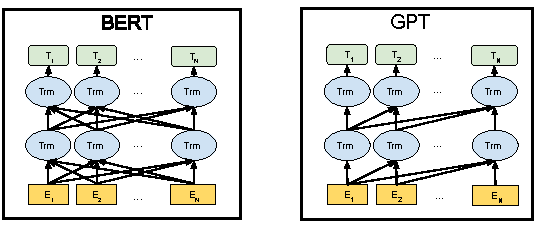
\includegraphics[width=0.8\textwidth]{figs/bertgpt.pdf}
    \caption{BERT \& GPT}
    {\footnotesize
    \textbf{BERT}: Bidirectional Encoder Representations from Transformers, used to create \textit{representations} of text;
    \textbf{GPT}: Generative Pre-training Transformer, used to \textit{generate} text.
    Their difference is whether the training is causal mode.
    }
    \label{fig:bertgpt}
\end{figure}